% Source: graduate-coursework/Sp26/CSCE775/Project/proposal_asv_3/proposal3_asv.tex
% Description: Evaluation pipeline. Six methods are evaluated across four water-body scenarios using five complementary metrics, yielding 120 method-scenario-metric combinations. Each combination comprises 100 independent trial episodes.

\documentclass[border=4pt]{standalone}
\usepackage{amsmath,amssymb}
\usepackage{pgfplots}
\usepackage{tikz}
\usepackage{xcolor}
\pgfplotsset{compat=1.18}
\usetikzlibrary{positioning, arrows.meta, shapes.geometric, fit, calc, backgrounds, patterns, decorations.pathreplacing}

\definecolor{Garnet}{HTML}{73000A}
\definecolor{Atlantic}{HTML}{466A9F}
\definecolor{Congaree}{HTML}{1F414D}
\definecolor{Horseshoe}{HTML}{65780B}
\definecolor{Rose}{HTML}{CC2E40}
\definecolor{Honeycomb}{HTML}{A49137}
\definecolor{Black90}{HTML}{363636}
\definecolor{Black70}{HTML}{5C5C5C}
\definecolor{Black50}{HTML}{A2A2A2}
\definecolor{Black30}{HTML}{C7C7C7}
\definecolor{Black10}{HTML}{ECECEC}
\definecolor{WarmGrey}{HTML}{676156}


\begin{document}
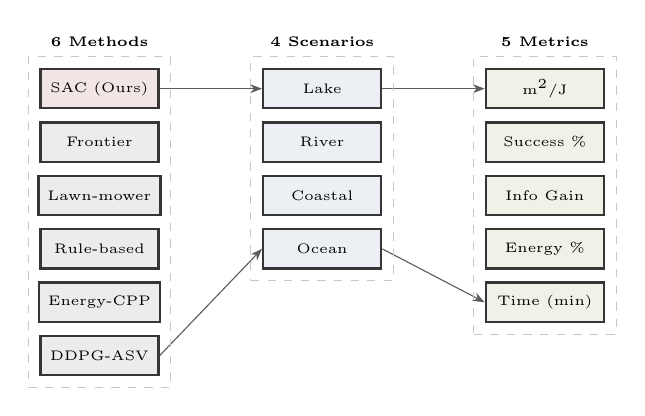
\begin{tikzpicture}[
    method/.style={draw=Black90, thick, minimum width=1.5cm, minimum height=0.5cm, align=center, font=\tiny},
    scenario/.style={draw=Black90, thick, minimum width=1.5cm, minimum height=0.5cm, align=center, font=\tiny, fill=Atlantic!10},
    metric/.style={draw=Black90, thick, minimum width=1.5cm, minimum height=0.5cm, align=center, font=\tiny, fill=Horseshoe!10},
    arr/.style={-{Stealth[length=1.5mm]}, color=Black70},
    every node/.style={font=\tiny}
]

% Methods column
\node[method, fill=Garnet!10] (m1) {SAC (Ours)};
\node[method, fill=Black10, below=0.15cm of m1] (m2) {Frontier};
\node[method, fill=Black10, below=0.15cm of m2] (m3) {Lawn-mower};
\node[method, fill=Black10, below=0.15cm of m3] (m4) {Rule-based};
\node[method, fill=Black10, below=0.15cm of m4] (m5) {Energy-CPP};
\node[method, fill=Black10, below=0.15cm of m5] (m6) {DDPG-ASV};

% Scenarios column
\node[scenario, right=1.3cm of m1] (s1) {Lake};
\node[scenario, below=0.15cm of s1] (s2) {River};
\node[scenario, below=0.15cm of s2] (s3) {Coastal};
\node[scenario, below=0.15cm of s3] (s4) {Ocean};

% Metrics column
\node[metric, right=1.3cm of s1] (k1) {m$^2$/J};
\node[metric, below=0.15cm of k1] (k2) {Success \%};
\node[metric, below=0.15cm of k2] (k3) {Info Gain};
\node[metric, below=0.15cm of k3] (k4) {Energy \%};
\node[metric, below=0.15cm of k4] (k5) {Time (min)};

% Connectors
\draw[arr] (m1.east) -- (s1.west);
\draw[arr] (m6.east) -- (s4.west);
\draw[arr] (s1.east) -- (k1.west);
\draw[arr] (s4.east) -- (k5.west);

% Cross-connections (implied by box)
\node[draw=Black30, dashed, inner sep=4pt, fit=(m1)(m6), label={[font=\tiny\bfseries]above:6 Methods}] {};
\node[draw=Black30, dashed, inner sep=4pt, fit=(s1)(s4), label={[font=\tiny\bfseries]above:4 Scenarios}] {};
\node[draw=Black30, dashed, inner sep=4pt, fit=(k1)(k5), label={[font=\tiny\bfseries]above:5 Metrics}] {};

\end{tikzpicture}
\end{document}
